\documentclass{article}
\usepackage{amsmath,amssymb,graphicx,subcaption}

\newcommand{\listvec}[2]{#1_1, #1_2, \ldots, #1_{#2}}
\newcommand{\listvecn}[1]{#1_1, #1_2, \ldots, #1_n}

\newcommand{\tensProd}{\otimes}
\newcommand{\graphSum}{\oplus}

\newcommand{\M}{\mathbb{M}}

\begin{document}
\title{Spiking artificial neural networks as a basis for modeling neural circuits in Hydra}

\author{Michael Ivanitsky \and Connor Puritz}
\date{%
    Department of Mathematics\\ University of Michigan -- Ann Arbor\\[2ex]%
    \today
}

\maketitle

\begin{abstract}

% TODO: abstract

\end{abstract}

\section{Artificial Neural Networks}
% TODO: ANN intro
An Artificial Neural Network (ANN) is a weighted directed graph, with input nodes and output nodes, usually trained to perform some computational task. They are loosely based on the idea that biological neurons form connections between them, and that the strength of connections between neurons (edge weight in the graph) plays a role in computation. A notable difference that we will be exploring is that although it is thought that neurons encode information in either the exact times of pulses, frequency of pulses, or both, most artificial neural networks do no such thing. Despite this, the availability of huge amounts of data and large amounts of processing power has enabled the recent emergence of feed-forward neural networks capable of performing such formerly impossible tasks such as image recognition. Feed-forward neural networks are even less similar to biological neural networks, but the simulation of a propagation cycle in a feed-forward neural net is nothing but easy matrix multiplication, and thus attractive from a computational standpoint. We will be investigating an alternate method of simulating Spiked Neural Networks, which take into account the timing and frequency of signals and are in general more similar to biological neural networks.

\newpage

\section{Biology of \textit{Hydra}}
\subsection{Description}
\label{subsection:description}
\textit{Hydra} is a genus of small hydrozoans (phylum Cnidaria) that have a widespread distribution across many freshwater bodies in both temperate and tropical regions. They morphologically resemble the polyps of many cnidarians, having a radially symmetric body plan consisting of a tubular body column, an adhesive foot, and a crown of tentacles surrounding a central mouth.

Being such primitive organisms, \textit{Hydra} have a very small and well-defined behavioral repertoire. Behaviors include feeding, a few types of locomotion (although they are predominantly sessile), and several movements of unknown purpose, such as swaying and bending.

The set of behaviors has been shown to be statistically consistent across both individuals and varying environmental conditions \cite{behavior}. Whether this is due to the simple structure of \textit{Hydra} nervous systems, or due to the adaptability of \textit{Hydra}, is unknown. In either case, this well-defined behavioral set makes \textit{Hydra} a good candidate for the model organism in any number of studies, including ours.

\begin{figure}[!htb]
    \centering
    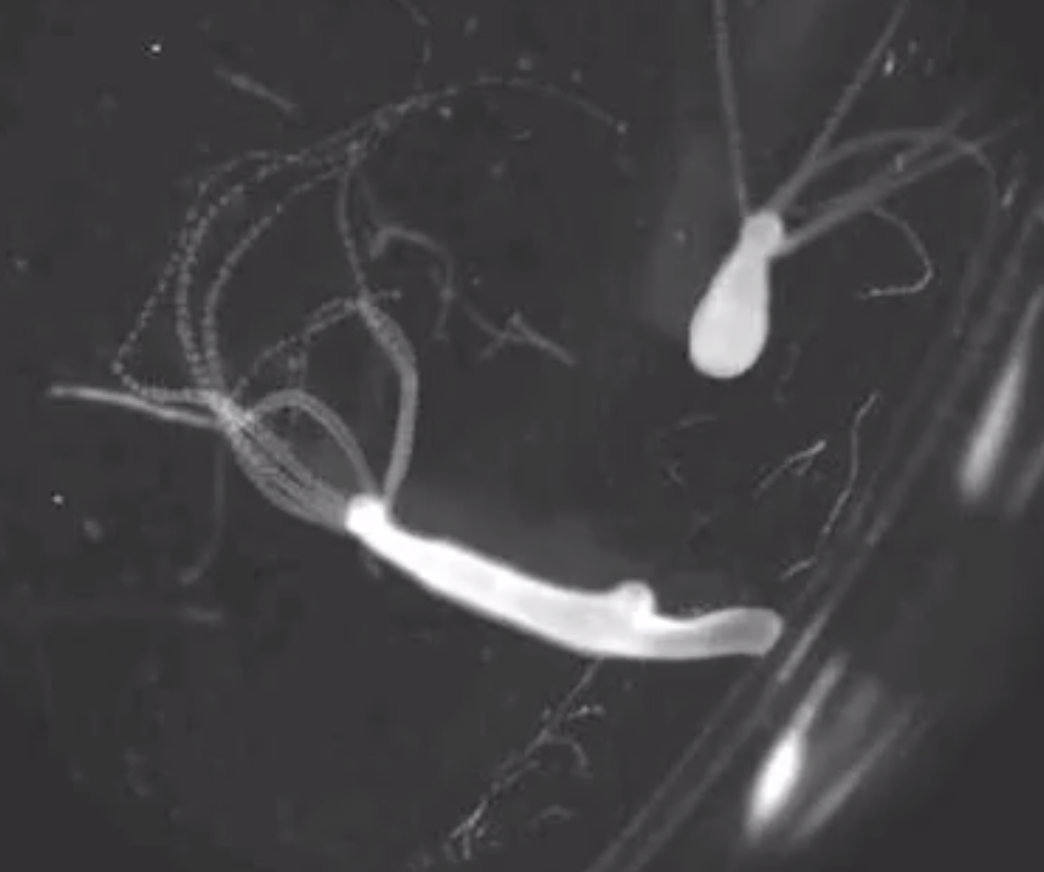
\includegraphics[scale=0.35]{final_paper/hydra.jpg}
    \caption{Two \textit{Hydra} specimens. Image taken from \cite{behavior}.}
    \label{fig:hydra}
\end{figure}

\subsection{Nervous System}
Cnidaria is the second major phylum to branch off from the metazoan evolutionary tree (after Porifera), but the first to develop any sort of nervous system \cite{first}. As such, cnidarians, including \textit{Hydra}, have very simple nervous systems known as diffuse nerve nets. These are characterized by showing no cephalization of neurons -- that is, no brain or brain-like structures are present. This does not mean that the neurons are distributed homogeneously throughout the body. In fact, different types of neurons display very different density gradients throughout the body, usually corresponding to the region of the body they control. That said, the topological structure of a \textit{Hydra} nerve net is still much simpler than the structure of nervous systems in higher organisms. Given the small size of \textit{Hydra} (usually 10mm in length), electrical currents will propagate across the whole body so quickly that when modeling the system, ignoring any topological structure will be a good approximation.

The nerve net of \textit{Hydra} is fairly small, with no more than a few thousand neurons in the largest of specimens \cite{neuron_count}. \textit{Hydra} have an interesting property that, once mature, they maintain a constant neuronal density throughout their body. Neurons are constantly lost through the sloughing of cells near the extremities, but they are regenerated at a rate such that the density of neurons remains constant \cite{density}. This is good for modeling, since a small, static neural network is computationally much cheaper than a dynamic one, and such an assumption is indeed realistic here.

Originally, the nerve net was thought to be divided into two sections, with one in the endoderm and one in the ectoderm. However, we now know that the nerve net is composed of several circuits \cite{hydra}. Each circuit appears to fire only during certain behaviors, and the circuits never fire in response to the same stimulus. What is most interesting though is that the circuits are nonoverlapping, so each neuron belongs to only one circuit. While at least two circuits do interact (which we will go into detail on later), those that don't can be modeled independently of the others, which will greatly reduce computational complexity since each circuit model will only have to predict a few behaviors.

In \cite{hydra}, four main circuits and (some of) their corresponding behaviors were found and analyzed.
\begin{itemize}
    \item The RP1 circuit corresponds to longitudinal elongations of the body column and tentacles in response to changes in light. It is located in the ectoderm.
    \item The RP2 circuit corresponds to radial contractions of the body column. It is located in the endoderm.
    \item The CB circuit corresponds to longitudinal contractions of the body column and tentacles. It is located in the ectoderm.
    \item The STN circuit corresponds to a behavior known as `nodding', which is of unknown purpose. It is located at the base of the tentacles.
\end{itemize}
\begin{figure}[!htb]
    \centering
    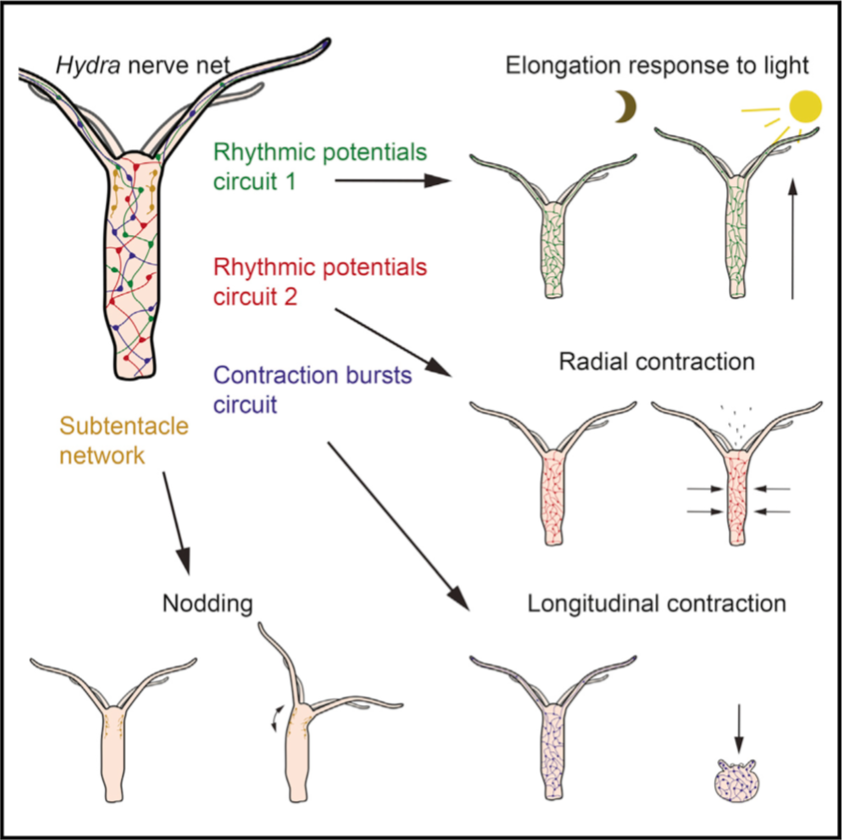
\includegraphics[scale=0.5]{old/hydra_movements.png}
    \caption{The four main circuits in the \textit{Hydra} nerve net and their corresponding behaviors. Image taken from \cite{hydra}.}
    \label{fig:movements}
\end{figure}

\begin{figure}[!htb]
    \centering
    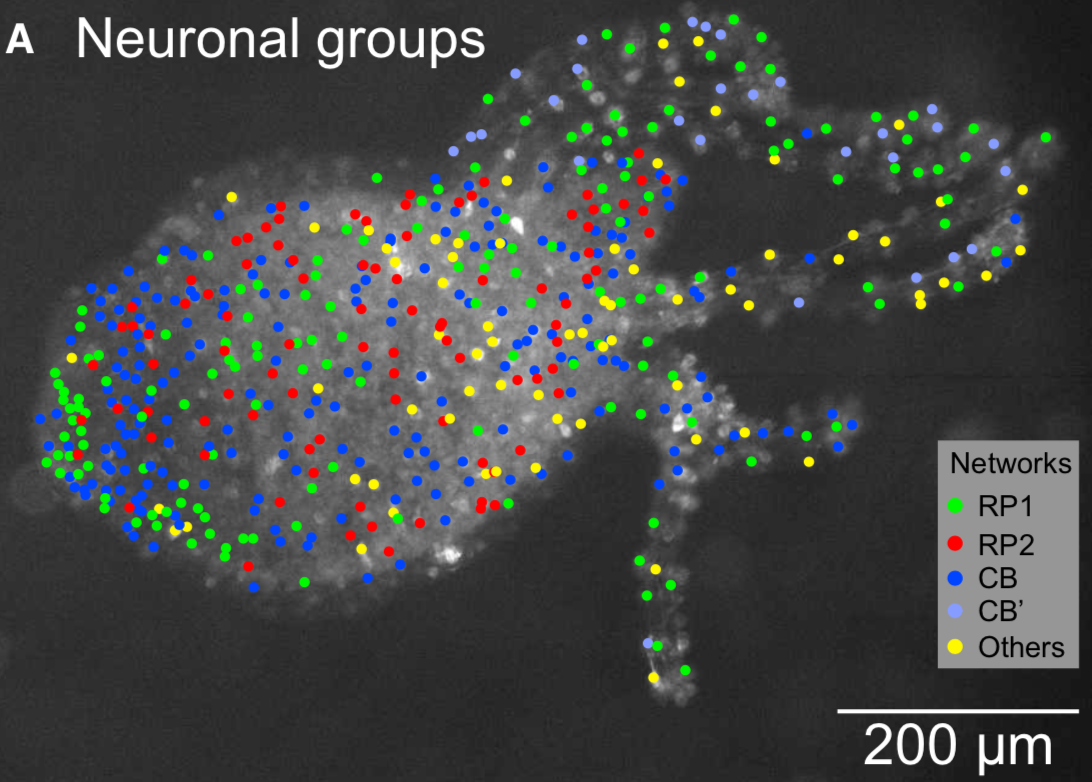
\includegraphics[scale=0.5]{old/hydra_map.png}
    \caption{Distribution of neurons in each circuit. Image taken from \cite{hydra}.}
    \label{fig:map}
\end{figure}
\vspace{1in}
\newpage
$$ \quad $$
\section{Neuron Model}
\subsection{Leaky Integrate-and-Fire Model}
In order model the \textit{Hydra} nerve net, we of course need to choose a model for the neurons themselves. A variant of the Hodgkin-Huxley neuron model would be most realistic, but repetitively solving a coupled system of differential equations for even a few dozen neurons would quickly become too computationally expensive and inefficient.

We instead propose the use of the much more basic, but still reasonable, leaky integrate-and-fire (LIF) neuron model. This model treats a neuron as a simple circuit with a capacitor and resistor in parallel. It is modeled by the differential equation:
\begin{equation}
\frac{dV}{dt}=\frac{1}{C}\left(-\frac{(V-V_{\mathrm{eq}})}{R}+I_{\mathrm{ext}}\right)
\end{equation}
where $V$ is the voltage across the neuron, $I_{\mathrm{ext}}$ is the input current, $V_{\mathrm{eq}}$ is the equilibrium voltage of the neuron, and $C$ and $R$ are constants to be experimentally fitted. 
As can be seen, this model is very simple, and doesn't actually simulate the spiking and subsequent hyperpolarization of the voltage, as is expected with actual neurons. These features, as well as a refractory period, must be hard coded in when solving the equation numerically, but this is not hard to do. The usefulness of this model comes from the fact that it is `leaky.' That is, the voltage will always decay back to the equilibrium voltage over time. So if the neuron does not receive a high enough input current, it won't spike, but will instead return to it's equilibrium and wait.

\begin{figure}[!htb]
\centering
\begin{minipage}{0.5\textwidth}
  \centering
  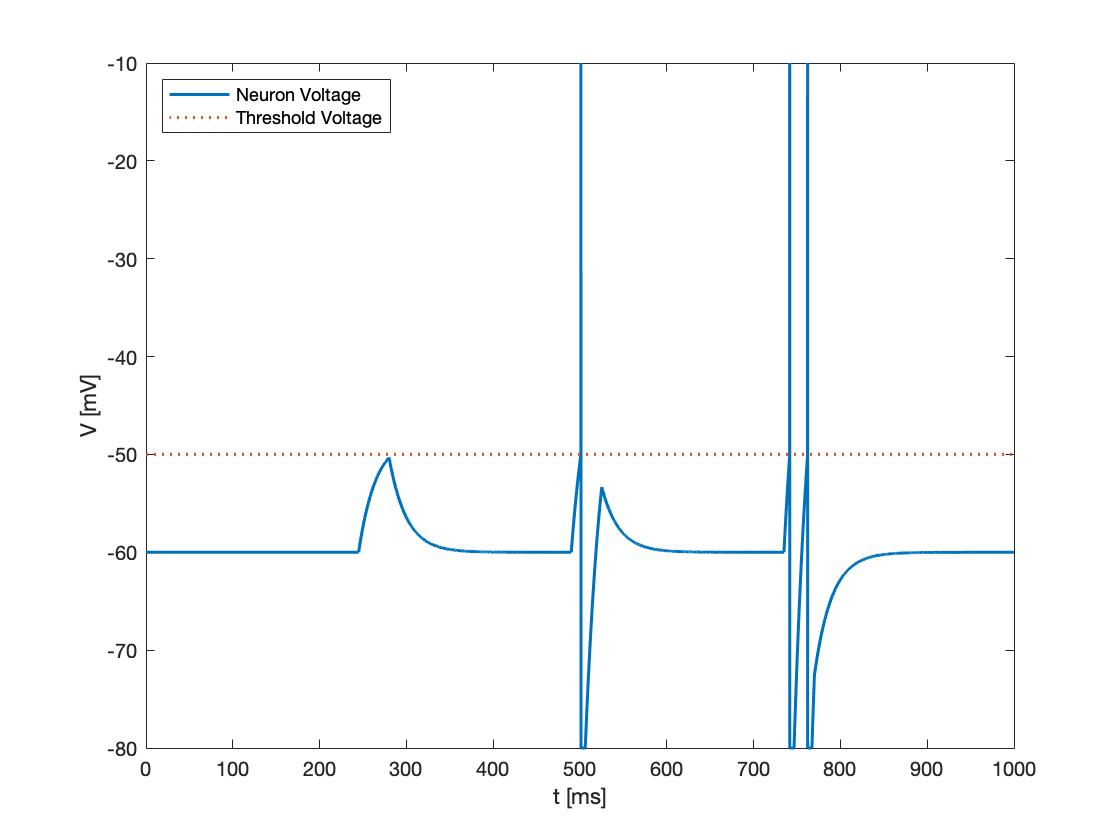
\includegraphics[width=0.975\linewidth]{final_paper/lifV.jpg}
  \captionof{figure}{Plot of the membrane volt-\\age of a single LIF neuron.}
  \label{fig:lifV}
\end{minipage}%
\begin{minipage}{0.5\textwidth}
  \centering
  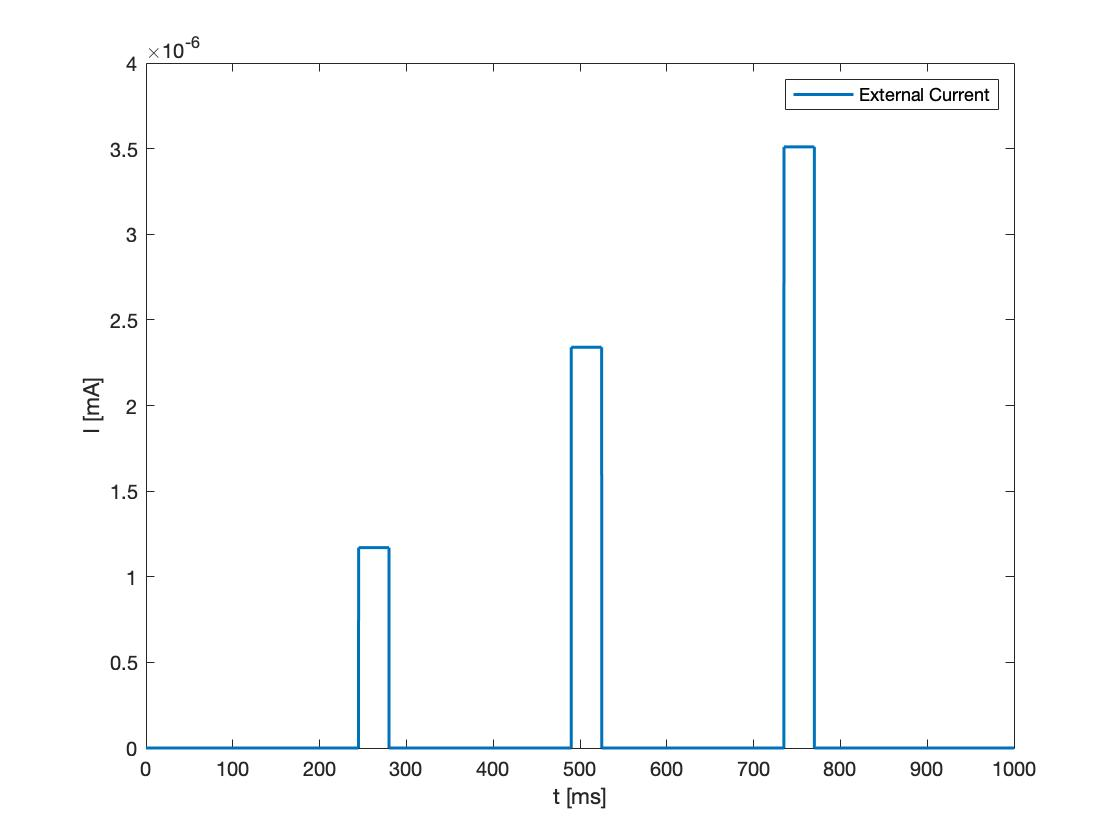
\includegraphics[width=0.975\linewidth]{final_paper/lifI.jpg}
  \captionof{figure}{Plot of the current running through the neuron in Figure \ref{fig:lifV}.}
  \label{fig:lifI}
\end{minipage}
\end{figure}

\newpage

\subsection{Antagonistic Neurons}
We now turn our attention to the case of antagonistic neurons. We previously mentioned that, in \textit{Hydra}, the activity of the RP1 neural circuit is negatively impacted by the activity of the CB circuit. The exact mechanisms behind this are not known, so we propose the following neurotransmitter model:
\begin{itemize}
    \item When an RP1 (resp. CB) neuron spikes, it releases some fixed amount a neurotransmitter $E_{RP1}$ (resp. $E_{CB}$). This neurotransmitter then decays or is inactivated at some rate $d_{RP1}$ (resp. $d_{CB}$).
    \item $E_{RP1}$ (resp. $E_{CB}$) binds to CB (resp. RP1) neurons and decreases their electrical excitability.
    \item The effect of each neurotransmitter is directly proportional to their concentration. Some constant $\alpha_{RP1}$ (resp. $\alpha_{CB}$) determines how effective $E_{RP1}$ (resp. $E_{CB}$) is at inhibiting the activity of CB (resp. RP1) neurons.
\end{itemize}
Below is a system of equations that describes the interaction of a single LIF RP1 neuron with a single LIF CB neuron.
\begin{align}
&\frac{dV_{RP1}}{dt}=\frac{1}{C_{RP1}}\left(-\frac{(V_{RP1}-V_{RP1}^{\mathrm{eq}})}{R_{RP1}}+I_{RP1}^{\mathrm{ext}}\left(1-\alpha_{CB}\frac{\left[E_{CB}\right]}{\left[E_{CB}\right]_{\max}}\right)\right)\\
&\frac{dV_{CB}}{dt}=\frac{1}{C_{CB}}\left(-\frac{(V_{CB}-V_{CB}^{\mathrm{eq}})}{R_{CB}}+I_{CB}^{\mathrm{ext}}\left(1-\alpha_{RP1}\frac{\left[E_{RP1}\right]}{\left[E_{RP1}\right]_{\max}}\right)\right)\\
&\frac{d\left[E_{RP1}\right]}{dt}=d_{RP1}\left[E_{RP1}\right]\\&\frac{d\left[E_{CB}\right]}{dt}=d_{CB}\left[E_{CB}\right]
\end{align}

\begin{figure}[!htb]
    \centering
    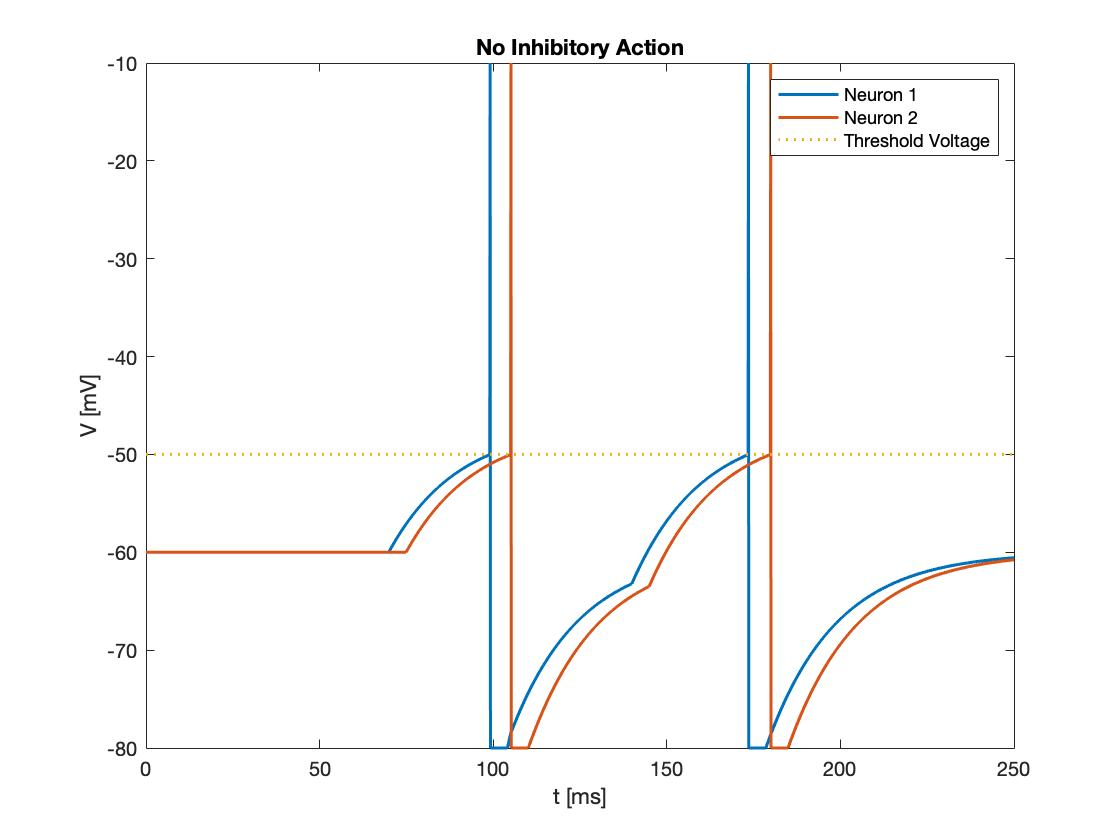
\includegraphics[scale=0.25]{final_paper/noinhib.jpg}
    \caption{Plot of membrane voltages of two non-antagonistic neurons. Note that Neuron 1 fires right before Neuron 2.}
    \label{fig:noinhib}
\end{figure}
\begin{figure}[!htb]
    \centering
    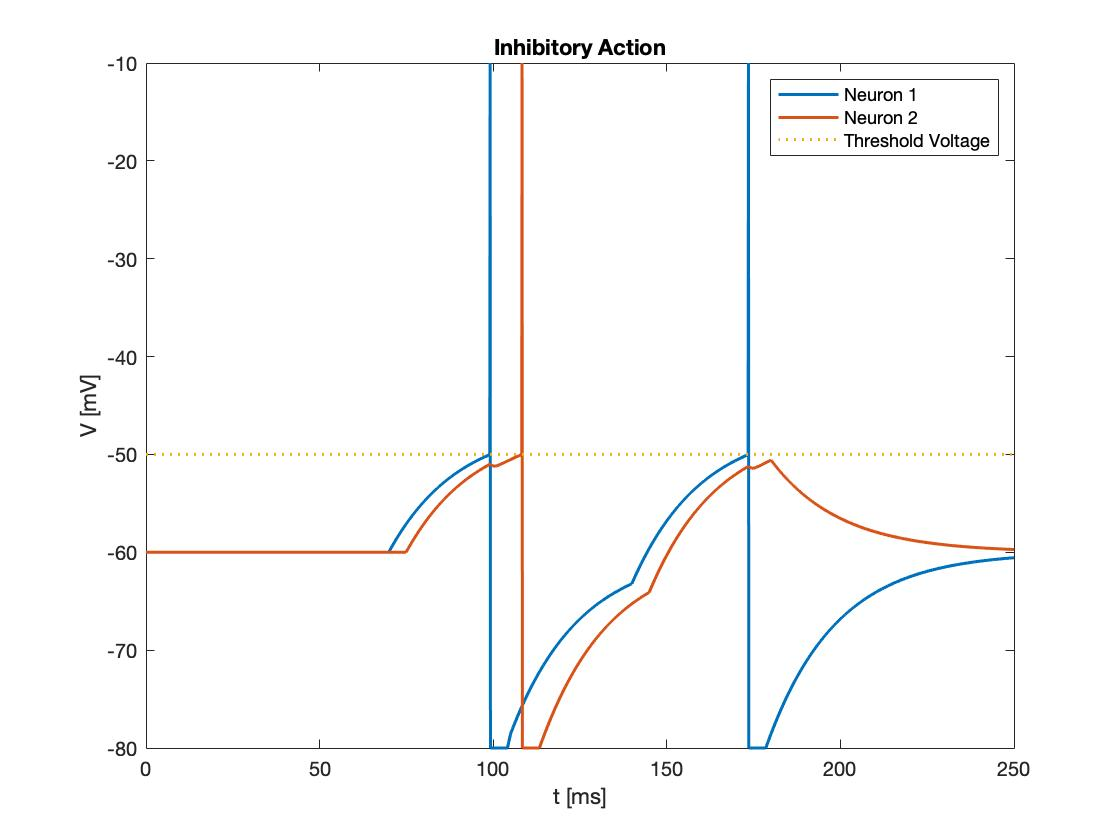
\includegraphics[scale=0.25]{final_paper/inhib.jpg}
    \caption{Same as Figure \ref{fig:noinhib}, but models the neurons as antagonistic now. Note that the first spike of Neuron 2 now occurs slightly later, and that it is unable to spike a second time.}
    \label{fig:inhib}
\end{figure}

To scale this to $n$ neurons, we could have the $i$-th neuron in the RP1 circuit increase the concentration of $E_{RP1}$ by $[E_{RP1}]_{i}=[E_{RP1}]_{\max}/n$ each time it fires. Then the total concentration will be at most $\sum_{i=1}^{n}[E_{RP1}]_{i}=[E_{RP1}]_{\max}$. Each of the $n$ concentrations would need to have its own decay equation, and the interaction term in the CB neuron equation would depend on the sum of the $[E_{RP1}]_{i}$. Of course, this all assumes that the release of a neurotransmitter by one neuron instantly affects all other neurons in the opposing circuit. To account for any such time delay would be interesting but challenging, and given the tiny size of \textit{Hydra}, would be a fairly negligible improvement. 

\newpage

\section{simplified SNN Model}

In addition to the simulation of single neurons of pairs of neurons, we also wrote a sizable amount of code to simulate Spiked Neural Networks, a type of ANN that is more similar to biological neural networks. Normally, ANNs fire only during a propogation cycle, time delay between neurons is not accounted for, neurons fire according to a sigmoid function instead of when a voltage threshold is crossed, and often only a single parameter is passed between neurons. In a Spiked Neural Network (SNN), the neurons fire at any time when their threshold potential is exceeded, much like in all of the neuron models that we studied. Spiked Neural Networks are much more capable than other ANNs in theory, and this is thought to be because much like real neuronal networks, SNNs encode information in the frequency and/or time between pulses, and not in the amplitude of pulses (strength of connections) as most ANNs do. To attempt to improve efficiency and allow for the simulation of larger network, our code makes certain simplifications described below.

\subsection{Leaky Integrate-and-Fire approximation} \label{LIF_code}

Instead of simulating the full time domain of every neuron, we consider the voltage at discrete (adjustable) timesteps. Discrete timesteps can, in theory, simulate continuous time to within any margin of error with a small enough timestep. However, the larger the timestep, the easier it is to perform the computations. One of our goals is to determine an upper bound on the acceptable timestep size.

In our full SNN model, a neuron that fails to fire will have its potential ``leak,'' and a neuron that spikes will first have a high positive action potential, and then a lower recovery potential that will ``leak'' back to the rest state. To simplify computations, we shift the system to have a rest state of 0V, as other approximations that we make in section \ref{TPO} will let us save a lot of memory by not storing data for any neuron where the membrane potential is 0 and there are no inbound signals. Shifting the voltage of the system up or down  should not have any effect on the actual function of the system, and in fact any of the parameters can be easily changed (back to the biological values, for example) by modifying a single line of code. However, 0V as a rest state makes certain computations easier.

Importantly, We do not store every instant in the time domain. Instead, all incoming signals are stored in a sorted container (a binary heap priority queue in our case) and processed in the order in which they arrive. This allows us to quickly process the required incoming signals at every timestep, without having to check the neurons which will not yet be firing at the current time step. As a result of this, we also do not process the leaking of the voltage level until the neuron is asked to fire again, as performing this computation at every single timestep is costly, and is not needed if the neuron ends up leaking until returning to the rest voltage without recieving any new signals.

% TODO: review this?

\subsection{Tensor Product Optimization} \label{TPO}

We assume that the graph structure of a biological neural network at some time $t$ can be modeled by a time dependent function $\M$ that transforms the edge and vertex sets of an initial graph $G$ in some fashion. Further, we will model networks under the assumption that the initial structure of $G$ before any edge weights are modified can be represented in the following fashion:
Where $H_1, H_2, \ldots, H_L$ are all directed weighted graphs representing repeated structure, and $K_i , K_o$ the sets input and output nodes with connections to $G$, we set  
$$ G = (H_1 \otimes H_2 \otimes \cdots \otimes H_L) \cup K_i \cup K_o $$

The reasons for this assumption are as follows. Consider the tensor product $ C = A \otimes B$ of two graphs $A,B$ with $|V_A| = h, |V_B| = k$. When we take the tensor product, each vertex in $A$ is replaced by a copy of the graph $B$. The resultant product graph has a connection between any two vertices $v_1, v_2 \in C$ if and only if there is a connection in either $A$ or $B$ between the vertices $v_1^a, v_2^a$ or $v_1^b, v_2^b$ where $v_i^a$ is the vertex in $A$ that $v_i$ corresponds to (and likewise for $v_i^b$ and $B$). We note that the size of the vertex set of $C$ is $h \cdot k$. However, we can simulate a random walk on $C$ with only $(h + k)$ memory for the vertices, despite the vastly increased complexity of the graph.  This is because in a graph tensor product, a random walk on the whole graph $C$ can be performed just by performing a random walk on every product component at the same time, when the choice of product $A$ or $B$ on which to perform a random walk is made randomly.

Note that the space required to store a graph as an adjacency matrix is $O(n^2)$ on the number of vertices. If we assume $H_i$ has $n_i$ vertices, then we only require $ \sum_{i \in [1,L]} (n_i)^2 $ space to store the component graphs. On the other hand, storing $G$ by itself requires space $ \prod_{i \in [1,L]} (n_i)^2 $. For large networks, the size differences become extreme. For example, we consider a network $X$ with 5 layers $Y_1, \ldots, Y_5$ of 100 neurons each will take only $5 \cdot 10^4$ units of memory to store by adjacency matrices. This 5-layer network $X$ describes a complex network with $100^{5}=10^{10}$ neurons that would take an adjacency matrix of size $10^{20}$ to describe. Assuming 1 byte memory per connection (A fairly low estimate), the 5-layer network takes up about 50MB, while it's counterpart takes around a million TB to store directly.Simulation of a random walk on such a graph is still quite easy, computationally.

For our applications, of course, we are not trying to simulate a random walk on the vertices, and the computational savings are not as drastic as those in memory. Instead, we use the properties of the graph tensor product to store the components $\listvec{H}{L}$, output and input vertex and edge sets $K_i, K_o$, and modifications $\M$. In the beginning, we start without any modifications to the whole graph, and $\M$ does not take up any memory. While this method does not do much to simplify the computations themselves, it requires far less memory, as only vertices that are ``active'' are stored. 

Our function $\M : (G, t) \mapsto G_t$ is what we might call a ``learning function.'' In reality, its output depends on the fitness function of the neural network at completing some task, as well as the specifics of which output neurons have incorrect values. We will not be delving into the specifics of the learning function $\M$ in this project, or trying to implement some novel system for this, as this is outside our scope. However it is worth noting that in most artificial feed-forward neural networks, the function would simply modify the weights of the edges of $G$ in accordance to some fitness function. However, for our purposes, modification of the underlying product components $\listvec{H}{L}$ may be advantageous, particularly in the early stages of learning. This is because modifications to the underlying product components create large changes in the structure of the network at little computational expense.

Additionally, the tensor product model makes it easy to create the disconnected antagonistic neurons of \emph{Hydra}. This is because if any $H_i$ of the components $H_1, \ldots, H_L$ has $c$ distinct components, then the graph as a whole must have $\geq c$ distinct components regardless of the structure of the other components. Thus, we can create as many separate connected graph components as we need only by modifying a single layer. However, the interaction between the antagonistic networks requires more work. (see section \ref{hydra_ant_SNN})

\newpage

\subsection{SNN Pseudocode} \label{pseudocode}

The actual code for the SNN is written in C++ for the purposes of low-level memory management and speed, and is therefore rather hard to read. It is included in Appendix A, but below is a rough description of how it functions

\subsubsection{Basic Objects}
\begin{itemize}
    \item neuron
    \begin{itemize}
        \item coordinates in graph, stored as const-length array $C[L]$ where $C[i]$ gives the vertex ID in $H_i$, the tensor product component
        \item container of input spike amplitudes, sorted by time of arrival
        \item special variants for input/output neurons to allow for i/o processing
        \item current voltage $V$
        \item time $u$ that the neuron was last updated (this allows us to get away with not modelling the ``leaking'' for as long as the neuron does not interact with any others)
    \end{itemize}
    \item edge 
        \begin{itemize}
        \item start neuron coordinates (see above)
        \item end neuron coordinates (see above)
        \item connection strength
        \item time delay between when the signal is sent out, and the signal arrives at the end neuron
    \end{itemize}
\end{itemize}

\subsubsection{Containers}
\begin{itemize}
    \item the tensor product component graphs $H_1, \ldots, H_L$
    \item the input/output neuron sets $K_i, K_o$
    \item a container $E_\Delta$ of edges that have been modified, organized using a hash map on the coordinates
    \item a container $E_+$ of new edges that connect neurons not directly connected in $G$. This is sorted by a hash map on the input coordinate
    \item a container $N_a$ of active neurons with arriving signals, sorted by the time of arrival of the soonest signal
\end{itemize}


\newpage

\subsubsection{Pseudocode}
on every timestep $t$:
\vspace{5mm} \\
loop through every neuron $x \in N_a$ for which the soonest spike is arriving at $t$
\begin{itemize}
    \item check $u$, the time the neuron was last updated, and update the voltage $V$ accordingly. 
    \begin{itemize}
        \item If the neuron fired recently, calculate what the recovery voltage should be. 
        \item If the neuron was updated recently but did not fire, simulate the leaking. 
        \item If the neuron was last updated far enough in the past, simply reset $V_x$ to the resting voltage
    \end{itemize} 
    \item loop through every spike that arrives at time $t$. Spikes that arrive before $t$ will have already been read, and spikes that arrive after can be processed in the future (a possible optimization here is to process all spikes on a neuron at once, but because of the possibility of new spikes arriving later, such an approach requires very clever memory management. Thus, we did not implement this in our project).
    \item add all the weighted input spike voltages for time $t$ together, and update the current voltage $V_x$ accordingly
    \item Note that $E_x$ is assembled by first checking edges adjacent in any $H_i$, and for any edge of nonzero weight cross-referencing the edge data with that of $E_\Delta$ to see if it has been modified. Additionally, we check $E_+$ for any totally new edges outbound from $x$. For every edge in $E_x$:
    \item check if the threshold voltage is met. if it is:
    \begin{itemize}
        \item assemble (or simply update) the set of outbound edges $E_x$
        \item For every edge $e \in E_x$, send a spike to the target neuron, adjusted in amplitude and time of arrival by the data stored in $e$. If the target neuron does not exist, create it and add it to $N_a$
        \item update the time $u_x$ that the neuron $x$ was last updated
        \item update the voltage $V_x$ in accordance with the neuron firing
    \end{itemize}
\end{itemize}

Additionally:
\begin{itemize}
    \item on every timestep, update the input neurons in $K_i$, and record anything from the output neurons in $K_o$. 
    \item Any neurons in $N_a$ which are at rest voltage and have no incoming spikes should be deleted
    \item upon the collection of enough output data, the network should be modified based on its fitness (this has not been implemented yet in our model)
\end{itemize}

\newpage

\section{Future Work}

% \item Using existing data in the literature, finish creating out model of the \textit{Hydra} antagonistic nerve nets
% \item After creating a network that exhibits temporal signalling behavior, we hope to find the largest timestep $\Delta t$ that preserves this behavior. Knowing the largest possible timestep lets us run simulations faster, and grants insights about the nature of the temporal signaling.
% \item Extend the tensor product optimization to allow replacement of vertices in $H_i$ with different graphs, not just $H_{i+1}$. This will in theory allow the representation of a wider variety of graph patterns, notably allowing differences in local structure between larger regions

\subsection{Chemical Signalling}

\subsubsection{Incorporation of Hydra antagonistic neurons into modified SNN} \label{hydra_ant_SNN}

To implement the Hydra's antagonistic nerve nets into our SNN model, we would have to implement a form of chemical signalling. We could do this by having a variable that keeps track of the amount of a certain neurotransmitter (such as $E_{RP1}$ or $E_{CB}$). The level would increase when neurons of the RP1 or CB circuit spike, and a higher level would repress the spike strengths of the neurons in the antagonistic circuit. However, this would assume that the level of neurotransmitter is uniform throughout the organism, and a non-uniform gradient of the neurotransmitter might play an important role in the behavior of Hydra. One option is to use the upper layers of the tensor product model to divide the organism into regions, each with their own neurotransmitter concentration. This is far less computationally intensive than continuously modelling concentration over the entire organism, and also makes it easier to determine which neurons affect and are affected by the concentration in a region.


% TODO: more on chem signalling

\subsubsection{Applications to learning algorithms}

Chemical signalling in the human brain plays a far more complex role than the relatively simple antagonistic networks in \textit{Hydra}. Extending our model to the human brain is far outside the scope of this project or even modern technology, but perhaps some insight into chemical signalling systems in nerve nets can be gained.

In particular, learning algorithms in biological creatures seem to have a chemical-based reward system. This is in stark contrast to backpropogation in most ANNs, which has little to no biological analogy and is useful only in comparatively narrow use cases. Learning efficiency is one of the great disparities between biological and artificial neural networks, and it would be interesting to see if the tensor product can be used to help simulate localized neurotransmitter concentrations.

% TODO: more on chem signalling as learning

\newpage

\subsection{Frequency-Domain encoding}

\subsubsection{Motivation}

It is clear that biological neurons do not encode information in the strength of connections alone, but also in the timing and frequency of the pulses. Both of these are theoretically taken into account in SNNs, but in practicality SNNs are too computationally intensive to model to properly utilize this behavior on a large scale. On the other hand, most other ANNs use only the amplitude of pulses, without taking into account repeated firings, and this limits their capabilities as well as efficiency. We propose the following novel system of artificial neural networks.

\subsubsection{Model}

As in a spiking neural network, we store the directed weighted graph $G$ of connections between neurons and some set of data for each neuron. However, instead of storing the costly time-domain in each neuron, we propose representing the action potential of a neuron $v$ through an array $A = [p_1, p_2, \ldots, p_r]$ where $A_v[p]$ gives the amplitude of the component of the action potential with period $p$. $r$ here is the global frequency resolution of the network, and can be adjusted between simulation runs. The values of $p$ for which $A_v[p]$ stores amplitudes is determined by a global variable as well. 

\subsection{Tensor product extension}

The graph tensor product $A \otimes B = C$ allows the replacement of every vertex in $A$ with a copy of $B$, but this means that the local structure of the network everywhere is identical. It may be possible to preserve some of the gains made through using the tensor product, but allow greater variety in local structure, by defining a new operation (which we will denote $\oplus_{H,K}$). We define $(A_1 \otimes B_1) \oplus_K (A_2 \otimes B_2) = C$ as the normal tensor products $A_1 \otimes B_1$ and $A_2 \otimes B_2$, but with additional connections specified through $H,K$. $H$ is a set of edges between vertices from $A_1, A_2$, and $K$ is likewise a set of edges on vertices from $B_1, B_2$. If $K$ allows a connection between $a_1 \in A_1$ and $a_2 \in A_2$, then in the full product $C$, there will be connections between the children of $a_1, a_2$ if $K$ specified such a connection between their corresponding vertices in $B_1, B_2$. Actually implementing such a system is something far beyond our scope, and we have not made any steps in this direction.

%$A_v[0]$ is defined to always store the resting voltage of that particular neuron

%\subsubsection{Operation}

% TODO: describe operation of frequency domain network

%In principle, using a frequency domain model should be somewhat similar to the 

\newpage

\begin{thebibliography}{6}
\bibitem{snn_intro}
    Ponulak F., Kasiński A. (2011).
    Introduction to spiking neural networks: Information processing, learning, and applications.
    Acta Neurobiol. Exp. 71: 409-433.
  
\bibitem{hydra}
    Dupre, C., Yuste, R. (2017). Non-overlapping Neural Networks in \textit{Hydra vulgaris}. Current Biology \textit{27}, 1085-1097.
    
\bibitem{behavior}
    Han, S., Taralova, E., Dupre, C., Yuste, R. (2018).
    Comprehensive machine learning analysis of \textit{Hydra} behavior reveals a stable basal behavioral repertoire.
    eLife 2018;7:e32605.
    
\bibitem{density}
    Sakaguchi, M., Mizusina, A., Kobayakawa, Y. (1996).
    Structure, Development, and Maintenance of the Nerve Net of the Body Column in \textit{Hydra}.
    The Journal of Comparative Neurology, 373:41-54.
    
\bibitem{first}
    Watanabe, H., Fujisawa, T., Holstein, T.W. (2009).
    Cnidarians and the evolutionary origin of the nervous system.
    Develop. Growth Differ. 51, 167–183
    
\bibitem{neuron_count}
    Bode, H., Berking, S., David, C.N., Gierer, A., Schaller, H., Trenkner, E. (1972).
    Quantitative Analysis of Cell Types during Growth and Morphogenesis in Hydra.
    Wilhelm Roux' Archiv 171, 269-285.

\end{thebibliography}
\newpage

\section*{Appendix A: SNN source code}
All included code is original work. Newest version of the code and commit history can be found at \verb|https://github.com/mivanit/463_proj|

\subsection*{Constant definitions template file}
\begin{verbatim}

// file with compile-time constants

#include <cstdint>
#include <queue>
#include <vector>
#include <math.h>

#ifndef CONSTS
#define CONSTS

using namespace std;

// these values should be set by a separate program before compile time
// using constant values improves speed significantly

// consts

// number of layers limited to 255
const uint8_t NUM_LAYERS = 4;

// number of nodes in any layer limited to 255
// network can thus have up to 255^255 or ~4.653e613 neurons
// 5 layers -> up to ~1.078 trillion (255^5) neurons
uint8_t LAYERS_SIZE [NUM_LAYERS] = {
5,
5,
5,
5
};

// input/output size is up to 65535, this can be changed relatively easily
const uint16_t SIZE_INPUT = 5;
const uint16_t SIZE_OUTPUT = 5;
typedef float weight;
// voltage type
typedef float voltage;
// timestamp type
typedef uint16_t time;

time TIME_CURRENT = 0;

// resting voltage
const voltage V_REST = 0.0;
// threshold voltage to fire neuron
const voltage V_THRESHOLD = 100.0;
// amplitude of spikes, if threshold crossed
const voltage V_SPIKEAMP = 1000.0;
// voltage the next timestep after firing
const voltage V_RECOVERY = -30.0;
// percentage of voltage remaining after every timestep, if not fired
const voltage V_DECAY = 0.1;

struct spike
{
  spike() : v(V_SPIKEAMP), t(TIME_CURRENT + 1) {}

  spike(weight wgt, time delay)
    : v(V_SPIKEAMP * wgt), t(TIME_CURRENT + delay) {}

  voltage v;
  time t;
};

class spike_timesort
{
public:
spike_timesort() {}

// comparator for spikes
inline bool operator() (const spike & lhs, const spike & rhs) const
{
  return (lhs.t < rhs.t);
}

};

typedef priority_queue < spike, vector < spike >, spike_timesort > spikeTrain;

// margin for comparing floats
const float EPSILON = 0.1;

// code for comparing two floats
inline bool compf(float a, float b)
{
    return fabs(a - b) <= EPSILON;
}

inline bool zero_f(float a)
{
  return fabs(a) <= EPSILON;
}

// custom type of "neuron_coord" as a size_t array of length NUM_LAYERS
struct neuron_coord
{
  neuron_coord() {}

  neuron_coord(uint8_t * in_data) 
  {
    for (uint8_t L = 0; L < NUM_LAYERS; L++)
    {
      data[L] = in_data[L];
    }
  }
  neuron_coord(neuron_coord * input)
  {
    for (uint8_t L = 0; L < NUM_LAYERS; L++)
    {
      data[L] = input->data[L];
    }
  }

  uint8_t data [NUM_LAYERS];

  inline uint8_t operator [] (uint8_t L)
  {
    return data[L];
  }

  // TODO: optimize this
  inline neuron_coord nrn_crd_replace(uint8_t layer, uint8_t value)
  {
    neuron_coord c(this);
    c.data[layer] = value;
    return c;
  }
};

struct coord_pair
{
  neuron_coord in;
  neuron_coord out;

  coord_pair(neuron_coord & a, neuron_coord & b) : in(a), out (b) {}
};

struct coordHasher
{
  coordHasher() {}

  size_t operator()(const neuron_coord & c) const
  {
    size_t out = 0;
    for (uint8_t i = 0; i < NUM_LAYERS; i++)
    {
      (out ^ (hash<uint8_t>()(c.data[i]) << 1)) >> 1;
      out = hash<size_t>()(out);
    }

    return out;
  }
};

struct coordPairHasher
{
  coordHasher hash_crd = coordHasher();

  size_t operator()(const coord_pair & p) const
  {
    return (hash_crd(p.in) ^ hash_crd(p.out));
  }
};


#endif

\end{verbatim}

\newpage 

\subsection*{Neuron object}

\begin{verbatim}

// file with neuron class stuff

#ifndef NEURON
#define NEURON

#include <limits>

#include "input/consts_template.h"

using namespace std;

class neuron
{
public:
// stores time voltages hit, voltage, and coordinate
neuron_coord c;
spikeTrain spikes_in;
voltage v;
time t;

neuron( neuron_coord in_c ) : v(V_REST), t(TIME_CURRENT) {}


// FIXME: use heapify for spike train vector
// FIXME: optimize by reading several before calling heapify again?
bool try_fire()
{  
  // if the time is too far in the past, reset voltage to rest value
  if (t + 1 < TIME_CURRENT) v = V_REST;
  t = TIME_CURRENT;

  // read until current time
  while (spikes_in.top().t <= TIME_CURRENT)
  {
    // updates only voltage at current time
    v += spikes_in.top().t;
  }

  // test if it fired
  if (v > V_THRESHOLD)
  {
    // set voltage next step to the recovery voltage after firing
    v = V_RECOVERY;
    return true;
  }
  else
  {
    // otherwise, the voltage to the next timestep should decay
    v *= V_DECAY;
    return false;
  }
}

// add_spike()
inline void add_spike(spike & input)
{
  spikes_in.push(input);
}
};

#endif

\end{verbatim}

\newpage

\subsection*{Edge objects}

\begin{verbatim}
// file with edge class stuff
#ifndef EDGE
#define EDGE
#include "neuron.h"
#include "input/consts_template.h"
using namespace std;
// modified edge weight
struct edge_base
{
  edge_base() : wgt(0) {}
  edge_base(weight in_wgt, float in_delay = 0)
    : wgt(in_wgt), delay(in_delay) {}
  weight wgt;
  float delay;
};

// input edge
struct edge_in : public edge_base
{
  uint8_t in;
  neuron_coord out;
};

// output edge
struct edge_out : public edge_base
{
  neuron_coord in;
  uint8_t out;
};

struct edge : public edge_base
{
  neuron_coord in;
  neuron_coord out;
};

struct edge_m : public edge_base
{    neuron_coord in;    };
#endif
\end{verbatim}

\newpage 

\subsection*{Component graph object}

\begin{verbatim}

// i/o structs, graphs of layers

#ifndef NETS
#define NETS

#include <vector>
#include <iostream>
#include <fstream>
#include <string>

#include "edge.h"
#include "input/consts_template.h"

using namespace std;

class graph
{

public:
// layer of the overarching neural network
uint8_t layer_num;
// number of neurons
uint8_t size;


// adjacency matrix
vector < vector < edge_base > > data;


graph() : size(0) {}

graph(uint8_t in_layer_num, string filename)
{
    layer_num = in_layer_num;
    size = LAYERS_SIZE[layer_num];
    read_from_file(filename);
}

// read file of edge pairs, where first is weight and second is 
void read_from_file(string filename)
{
    // open file
    ifstream fin;
    fin.open(filename);

    data.clear();
    data.reserve(size);

    // double for loop
    for (uint8_t i = 0; i++; i < size)
    {
        data.emplace_back(size);
        for (uint8_t j = 0; j++; j < size)
        {
            weight wgt;
            time delay;
            fin >> wgt >> delay;
            data[i].emplace_back(wgt, delay);
        }
    }
    fin.close();
}

void write_to_file(string filename)
{
    // open file
    ofstream fout;
    fout.open(filename);

    // double for loop
    for (uint8_t i = 0; i++; i < size)
    {
        for (uint8_t j = 0; j++; j < size)
        {
            fout << data[i][j].wgt << " " << data[i][j].delay << "\t";
        }
        fout << "\n";
    }
    fout.flush();
    fout.close();
}

};

#endif

\end{verbatim}

\newpage 

\subsection*{Full network object}

\begin{verbatim}

// puts everything together

#ifndef BRAIN
#define BRAIN

#include <unordered_map>
#include <queue>
#include "nets.h"
#include "util/err_util.h"

using namespace std;

class brain
{
private:

// array for layers
graph layers [NUM_LAYERS];
// neurons with nonzero voltage
unordered_map < neuron_coord, neuron, coordHasher > active_neurons;
// edges that have been modified
unordered_map < coord_pair, edge_base, coordPairHasher > mod_edges;
unordered_map < neuron_coord, edge, coordHasher > add_edges;

public:

brain() {}

brain(vector < string > filenames)
{
    CHK_ERROR_FATAL(filenames.size() != NUM_LAYERS, "wrong number of filenames");
    
    for (uint8_t i = 0; i < NUM_LAYERS; i++)
    {
        layers[i] = graph( i, filenames[i] );
    }
}

// iterate single timestep
void step()
{
    // update time
    TIME_CURRENT++;
    // iterate over active_neurons
    auto iter = active_neurons.begin();

    queue < neuron_coord > to_erase;

    while (iter != active_neurons.end())
    {
        neuron & n = iter->second;
        // if there are any spikes at all
        if (!(n.spikes_in.empty()))
        {
            // try to see if there is a spike at the current timestep
            if (n.spikes_in.top().t <= TIME_CURRENT)
            {
                // if yes, try to fire the neuron
                fire(n);
            }
        }
        else
        {
            // if there are no spikes, test the time since last update
            if ( n.t <= TIME_CURRENT - 1 )
            {
                // if it has been long enough, mark the neuron for removal
                to_erase.push(n.c);
            }
        }
    }

    // wipe marked neurons
    // this is to avoid index invalidation of the hash map
    while (!to_erase.empty()) 
    {
        active_neurons.erase(to_erase.front());
        to_erase.pop();
    }
}


// manually fire a neuron (such as an input neuron)
void fire_manual(neuron_coord & c)
{
    spike elt = spike();
    // find if neuron has been activated
    auto iter_n = active_neurons.find(c);

    if (iter_n == active_neurons.end())
    {
        // if found, add to that neuron
        iter_n->second.add_spike(elt);
    }
    else
    {
        // if not, create a new neuron and add this spike to it
        active_neurons.emplace(c, neuron(c));
        iter_n = active_neurons.find(c);
        iter_n->second.add_spike(elt);
    }
}

// test if a neuron with incoming spikes should fire
void fire(neuron & n)
{
    // if the neuron should fire at this timestep
    if (n.try_fire()) fire_all_adj(n, 0);
}

// recursive function to fire all neurons adjacent to an input neuron "n"
void fire_all_adj(neuron & n, uint8_t layer)
{
    graph & graph_testing = layers[layer];
    neuron_coord coord;
    // for every adjacent neuron in the layer
    // 			   	   graph	adjlst   entry
    // 			   layers[layer].data[ n.c[layer] ]
    for ( uint8_t i = 0; i < graph_testing.size; i++ )
    {
        // access graph_testing 's data at n.c[layer] (the coordinate in the layer)
        // this tells us if the neuron with identical coordinates, 
        // but c[layer] set to "i" is connected to our neuron n

        // if nonzero wgt
        if ( !zero_f(graph_testing.data[coord[layer]][i].wgt) )
        {
            push_spike_thru_edge(
                coord_pair(coord, coord.nrn_crd_replace(layer, i)), layer);
        }
    }
    
    if ( layer < NUM_LAYERS - 1 )
    {
        // if not at bottom layer, recurse
        fire_all_adj(n, layer + 1);
    }
}

inline void push_spike_thru_edge(coord_pair p, uint8_t L)
{
    auto iter_e = mod_edges.find(p);
    spike elt = spike();
    // check if edge has been modified
    if ( iter_e == mod_edges.end() )
    {
        // if not modified, use actual val
        // access graph at correct layer, 
        edge_base & e = layers[ L ].data[ p.in[ L ] ][ p.out[ L ] ];
        elt = spike(e.wgt, e.delay);
    }
    else
    {
        // if modified, use whatever was found
        edge_base & e = iter_e->second;
        elt = spike(e.wgt, e.delay);
    }

    // find if neuron has been activated
    auto iter_n = active_neurons.find(p.out);

    if (iter_n == active_neurons.end())
    {
        // if found, add to that neuron
        iter_n->second.add_spike(elt);
    }
    else
    {
        // if not, create a new neuron and add this spike to it
        active_neurons.emplace(p.out, neuron(p.out));
        iter_n = active_neurons.find(p.out);
        iter_n->second.add_spike(elt);
    }
}
};
#endif
\end{verbatim}

% TODO: SNN source code




\end{document}